% !TEX root = ../main.tex

\chapter{Metodologia}
\label{Chapter3}

La metodologia aplicada en el desenvolupament de NUMEN ha estat un procés híbrid i evolutiu, adaptant-se a les necessitats canviants del projecte i a la corba d'aprenentatge personal. Aquest capítol detalla l'estratègia seguida des de la concepció inicial fins a la implementació final, així com les eines i recursos utilitzats.

\section{Estratègia de Desenvolupament}

El desenvolupament del projecte no ha seguit una línia temporal contínua i lineal, sinó que s'ha estructurat en diferents etapes marcades per la maduresa tècnica i la disponibilitat de temps.

\begin{figure}[h]
    \centering
    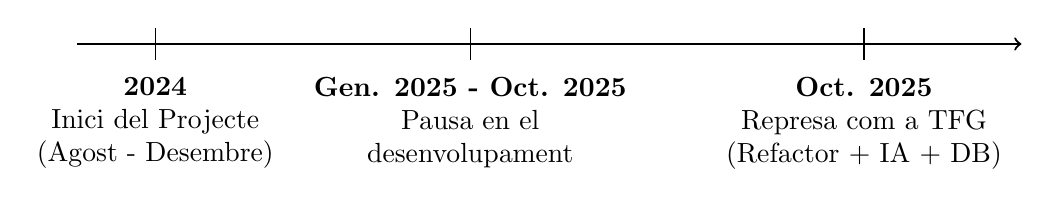
\begin{tikzpicture}
        % Draw the line
        \draw[thick, ->] (0,0) -- (12,0);
        
        % 2022 Node
        \draw (1,0.2) -- (1,-0.2);
        \node[align=center, below] at (1,-0.3) {\textbf{2024} \\ Inici del Projecte \\ (Agost - Desembre)};
        
        % 2023 Node
        \draw (5,0.2) -- (5,-0.2);
        \node[align=center, below] at (5,-0.3) {\textbf{Gen. 2025 - Oct. 2025} \\ Pausa en el \\ desenvolupament};
        
        % Oct 2025 Node
        \draw (10,0.2) -- (10,-0.2);
        \node[align=center, below] at (10,-0.3) {\textbf{Oct. 2025} \\ Represa com a TFG \\ (Refactor + IA + DB)};
    \end{tikzpicture}
    \caption{Línia temporal del desenvolupament del projecte NUMEN.}
    \label{fig:timeline}
\end{figure}

\subsection{Fase 1: Fonaments i Desenvolupament Inicial (2024)}
El projecte va néixer l'agost de 2024 amb una visió clara i una forta motivació personal. Durant aquest període, fins al desembre de 2024, el desenvolupament va ser continuat però intermitent, impulsat pel desig de ser productiu i ajudar a l'automatització dels càlculs manuals. En aquesta fase es va construir el nucli funcional de l'aplicació sense l'ús d'Intel·ligència Artificial.
En aquesta etapa inicial, el desenvolupament va ser purament manual i autodidacta. Sense l'assistència d'eines d'Intel·ligència Artificial, l'aprenentatge es va basar en la consulta de documentació oficial, tutorials en vídeo i l'estudi de patrons de disseny.

És important destacar que, en finalitzar aquesta etapa l'any 2023, \textbf{l'aplicació ja era completament funcional}. El sistema era capaç de realitzar tots els càlculs complexos, visualitzar les dades gràficament i generar informes imprimibles. Aquesta fita es va assolir exclusivament mitjançant la dedicació personal, a base de prova i error, i sense cap línia de codi generada per IA.
Aquest esforç manual atorga un valor afegit al projecte: tot i que avui dia eines com la IA Generativa permetrien aixecar un prototip similar en qüestió de dies, la robustesa i el control absolut sobre la lògica del nucli de NUMEN són fruit d'aquelles hores de programació artesanal.

\subsection{Fase 2: Recerca i Algorísmica}
Paral·lelament a l'aprenentatge tècnic, es va dur a terme una fase intensiva d'adquisició de coneixement del domini. La numerologia, segons el mètode de Martine Coquatrix, requereix una precisió matemàtica absoluta.
\begin{itemize}
    \item \textbf{Estudi Teòric:} Lectura i anàlisi profunda de l'obra \textit{La numerología a la luz del árbol de vida y las letras hebraicas}.
    \item \textbf{Consultoria Experta:} Col·laboració directa amb l'experta en la matèria (la meva mare), per validar regles complexes com la reducció de números mestres, el càlcul dels camins de vida o la interpretació dels números karmàtics.
\end{itemize}
Aquesta fase va culminar amb la implementació dels algoritmes de càlcul, transformant regles esotèriques en funcions lògiques deterministes.

\subsection{Fase 3: Integració Tecnològica i IA (Actualitat)}
En l'etapa final del projecte, s'han integrat tecnologies modernes per potenciar les funcionalitats existents. És en aquest punt on s'ha incorporat l'ús d'Intel·ligència Artificial Generativa, no per a la generació de codi base (ja consolidat), sinó com a component funcional del sistema (mòdul de \textit{prompting} i interpretació) i com a suport en la gestió de dades.

\section{Metodologia de Treball}
S'ha seguit una adaptació personalitzada de metodologies àgils. Donat que l'equip de desenvolupament està format per una única persona, s'ha optat per un enfocament iteratiu i incremental:
\begin{enumerate}
    \item \textbf{Disseny Inicial:} Definició de l'arquitectura i model de dades.
    \item \textbf{Implementació per Prioritats:} Codificació dels mòduls més influents i crítics (motor de càlcul) abans d'abordar la interfície d'usuari o la generació d'informes.
    \item \textbf{Refactorització Contínua:} Revisió constant del codi per millorar-ne l'eficiència i la llegibilitat a mesura que s'adquirien nous coneixements.
\end{enumerate}

\section{Declaració d'Ús d'Intel·ligència Artificial}
D'acord amb la normativa acadèmica i els principis de transparència, es declara explícitament l'ús d'eines d'Intel·ligència Artificial Generativa en aquest Treball Final de Grau.

\begin{itemize}
    \item \textbf{Desenvolupament de Software:} El nucli de l'aplicació, l'arquitectura i la lògica de negoci han estat desenvolupats manualment des de l'any 2024. L'ús d'IA en el codi s'ha limitat recentment a tasques de suport puntual, com la generació de consultes complexes a la base de dades o l'optimització de funcions específiques de \textit{prompting}.
    \item \textbf{Redacció de la Memòria:} S'han utilitzat models de llenguatge (com Google Gemini) com a assistents de redacció per a la revisió d'estil, correcció ortogràfica i estructuració de continguts, amb l'objectiu d'assolir un nivell de professionalitat i formalitat acadèmica excel·lent.
    \item \textbf{Autoria:} Tot el contingut generat o suggerit per la IA ha estat revisat, validat i editat exhaustivament, mantenint la responsabilitat total sobre la veracitat i originalitat del treball presentat. L'IA ha servit com a eina d'amplificació de capacitats, no com a substitut de l'autoria intel·lectual.
\end{itemize}
